\documentclass[
  utf8,%     More capable input encoding than latin-1.
  % parskip,%  For vertical whitespace between paragraphs.  This comes down to more than just using parskip.sty, so it's better to use this class option.
  % S5MP % If you intend to really use margin paragraphs (not recommended!).
%  crop,%     Produce output with crop marks and paper size A4.  Liu-Tryck should like this.  Automatically adds information, including the physical page number, at the top of each page.
       %     Add option 'noInfo' to suppress the info at the top of each page when using option 'crop'.
  % Font options: 'kp' (default), 'times', 'lm'.  The KpFonts (loaded using 'kp'), is the most complete font among the provided options.  Among other, it supports slanted small caps.  See rtthesis.cls for more details regarding the font options.
  largesmallcaps,intlimits,widermath,% Good options to KpFonts.
  sharecounter,nobreak,definition=marks,%  See comments in the results chapter of this document for more information on these options!
  %numbers, % If you want to cite references by numbers, use this option.
  noparts% Use option 'noparts' if you do not make use of part divisions.
]{rtthesis}

\usepackage{mythesis}

\begin{document}
\selectlanguage{english}
\frontmatter
\maketitle

\begin{abstract}[english]
  If your thesis is written in English, the primary abstract would go here while the Swedish abstract would be optional.

\end{abstract}

%!TEX root = main.tex
\begin{acknowledgments}
  Vi tycker alla har varit så himla goa hela den här långa och tuffa tiden i våra liv.

  \addvspace{1em}
  \begin{flushright}
    \textit{%
      Linköping, Januari 2020\\
      N N och M M%
    }
  \end{flushright}
\end{acknowledgments}


\tableofcontents
%!TEX root = main.tex
\begin{notation}% Passing the option "old" to the notation environment will redefine the notationtabular environment so that it produces an old style LaTeX tabular instead of a ctable.sty style tabular.
  \centering

  \begin{notationtabular}{Några mängder}{Notation}{Betydelse}
    $\naturals$ & Mängden av naturliga tal \\
    $\reals$ & Mängden av reella tal \\
    $\complexes$ & Mängden av komplexa tal \\
  \end{notationtabular}

  \begin{notationtabular}{Förkortningar}{Förkortning}{Betydelse}
    \abbrARMA\index{ARMA@\abbrARMA!abbreviation} & Auto-regressive moving average \\
    \abbrPID\index{PID@\abbrPID!abbreviation} & Proportional, integral, differential (regulator) \\
  \end{notationtabular}
\end{notation}


\mainmatter%

%!TEX root = main.tex
\chapter{Introduktion}\label{cha:intro}

\chapter{Resultat}\label{cha:Research}
%
Det här är kapitlet där resultaten presenteras.


\section{Ditten}\label{sec:research:history}
%
Liksom \citep{Duck:2005} har vi kommit fram till att glass smakar bäst på sommaren.

\marginpar{Kommer att tänka på en liten anekdot\ldots}

\Warning[TODO]{Ta bort den löjliga anekdoten!}

När vi nu går in på hur glass smakar vid olika tidpunkter under dagen hänvisar vi till \figureref{fig:times}, och speciellt till \figureref{fig:times:early}.  Jämför sedan med \figureref{fig:times2} för att se hur det kan bli när man äter glass vid okontrollerade tidpunkter.

Veselić, Krešimir (Veseli\'{c}, Kre\v{s}imir) skrev en gång en artikel med titeln \emph{Bounds for exponentially stable semigroups}.

\begin{figure}[tbp]
  \centering
  \subfloat[Alldeles för tidigt.][\label{fig:times:very-early}Det här är väl tidigt — din glass hinner smälta innan ditt sällskap dyker upp.]{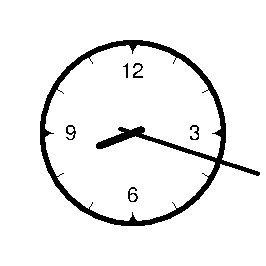
\includegraphics[page=1]{clocks}}
  \qquad
  \subfloat[Med marginal.][\label{fig:times:early}Kiosken stänger snart, men inte nu — perfekt!]{\includegraphics[page=2]{clocks}}
  \\
  \subfloat[I grevens tid.][\label{fig:times:on-time}Precis i tid — du får in ett finger i luckan just när kiosken ska stänga.  Han som jobbar blir sur, och det blir smolk i bägaren.]{\includegraphics[page=3]{clocks}}
  \qquad
  \subfloat[Försent.][\label{fig:times:late}Du är sen — kiosken är stängd.]{\includegraphics[page=4]{clocks}}
  \caption{\label{fig:times}%
    Illustration av \emph{subfloats}.  Den så kallade \emph{bounding box}en visas i \protect\subref{fig:times:late}.  Lägg märke till att bounding boxen har satts så att alla bilder har samma storlek, med enhetlig placering av själva innehållet i förhållande till bounding boxen.  Antag att du ska träffa en kompis för att äta glass just när kiosken stänger för dagen vid 08:30.  När dyker du upp?}
\end{figure}

\begin{figure}[tbp]
  \centering
  \subfloat[][\label{fig:times2:very-early}]{\includegraphics[page=5]{clocks}}
  \qquad
  \subfloat[][\label{fig:times2:early}]{\includegraphics[page=6]{clocks}}
  \\
  \subfloat[][\label{fig:times2:on-time}]{\includegraphics[page=7]{clocks}}
  \qquad
  \subfloat[][\label{fig:times2:late}]{\includegraphics[page=8]{clocks}}
  \caption{\label{fig:times2}%
    En andra illustration av \emph{subfloats}.  Den här gången har bounding boxen gjorts så liten som möjligt runt själva innehållet.  Resultatet är stökiga placeringar på sidan.  Samma sak kan hända med vanliga fyrkantiga figurer när man har text som spretar ut åt lite olika håll från själva rutan med kurvor i.}
\end{figure}

\section{Framtiden}

Sen när glassen är uppäten är det bara till att sätta igång och skriva på exjobbet igen!


\begin{chapter-appendix}

\section{Ett par långa bevis}
%
Det här är en appendix-del av det aktuella kapitlet.

\end{chapter-appendix}

\chapter{Avslutande kommentarer}\label{cha:conclusions}
%
Sätt av ett k asda  addwda kapitel sist i rapporten till att avrunda och föreslå rikningar för framtida utveckling av arbetet.

\part*{Appendix}
\appendix
%!TEX root = main.tex
\chapter{Trista saker}\label{cha:boring}
Långa beräkningar brukar bli rätt trista\dots

Detta är ett appendix-kapitel.  Jämför med appendixet i \chapterref{cha:Research}.

\section{Bädda sängen}

Den här beräkingen är så trista att vi kallar den \emph{att bädda sängen}.

\section{Diska}

Den här beräkingen är så trista att vi kallar den \emph{att diska}.


\clearemptydoublepage%

\backmatter%

\bibliography{IEEEfull,myrefs}

\printindex

\end{document}
